%%%%%%%%%%%%%%%%%%%%%%%%%%%%%%%%%%%%%%%%%%%%%%%%%%%%%%%%%%%%%%%%%%%%%%%%%%%%%%%
% PAPER
%%%%%%%%%%%%%%%%%%%%%%%%%%%%%%%%%%%%%%%%%%%%%%%%%%%%%%%%%%%%%%%%%%%%%%%%%%%%%%%

\documentclass[11pt]{paper}

% These go first.
\usepackage[T1]{fontenc}
\usepackage{fontspec}

% Hyperref comes before everything else.
\usepackage{hyperref}

% Everything else (order to be played with!).
\usepackage{amsmath}
\usepackage{amssymb}
\usepackage[
    sorting=none,
    backend=bibtex,
    style=numeric-comp
    ]{biblatex}
\usepackage{booktabs}
\usepackage{caption}
\usepackage{chemformula}
\usepackage{fancyvrb}
\usepackage{geometry}
\usepackage[
    symbols,
    nogroupskip,
    sort=none
    ]{glossaries-extra}
\usepackage{minted}
\usepackage{multirow}
\usepackage{paralist}
\usepackage{pgfplots}
\usepackage{setspace}
\usepackage{siunitx}
\usepackage[titles]{tocloft}
\usepackage{xfrac}

% This comes after other maths packages.
\usepackage{unicode-math}

%%%%%%%%%%%%%%%%%%%%%%%%%%%%%%%%%%%%%%%%%%%%%%%%%%%%%%%%%%%%%%%%%%%%%%%%%%%%%%%
% CONFIGURATION
%%%%%%%%%%%%%%%%%%%%%%%%%%%%%%%%%%%%%%%%%%%%%%%%%%%%%%%%%%%%%%%%%%%%%%%%%%%%%%%

% Make units detect font.
\sisetup{detect-mode}

% Set all math symbols to upright.
\unimathsetup{%
    math-style=upright,%
    bold-style=upright,%
    sans-style=upright,%
    nabla=upright,%
    partial=upright,%
}

% Configure fonts.
\setmainfont[Ligatures=TeX]{Calibri}
\setmathfont{Cambria Math}

% Make margins smaller.
\geometry{margin=20mm}

% Configure TOC.
\renewcommand{\contentsname}{Table of contents}
\renewcommand{\cftdotsep}{5}
\renewcommand{\cftsecdotsep}{5}
\renewcommand{\cftsecleader}{\bfseries\cftdotfill{\cftsecdotsep}}

% Configure hyperlinks.
\hypersetup{
    colorlinks = true,
    linkcolor = black
}

% Point to bibliography database.
\bibliography{../../../databases/references}

%%%%%%%%%%%%%%%%%%%%%%%%%%%%%%%%%%%%%%%%%%%%%%%%%%%%%%%%%%%%%%%%%%%%%%%%%%%%%%%
% DRAFT MODE
%%%%%%%%%%%%%%%%%%%%%%%%%%%%%%%%%%%%%%%%%%%%%%%%%%%%%%%%%%%%%%%%%%%%%%%%%%%%%%%

\newif\ifnotdraft
\notdraftfalse

%%%%%%%%%%%%%%%%%%%%%%%%%%%%%%%%%%%%%%%%%%%%%%%%%%%%%%%%%%%%%%%%%%%%%%%%%%%%%%%
% COMMANDS
%%%%%%%%%%%%%%%%%%%%%%%%%%%%%%%%%%%%%%%%%%%%%%%%%%%%%%%%%%%%%%%%%%%%%%%%%%%%%%%

\DeclareSIUnit\atm{atm}
\DeclareSIUnit\scfm{SCFM}
\DeclareSIUnit\Normcubicmeter{Nm^3}

\newcommand{\openitem}{\item[$\square$]}
\newcommand{\markitem}{\item[$\boxtimes$]}

%%%%%%%%%%%%%%%%%%%%%%%%%%%%%%%%%%%%%%%%%%%%%%%%%%%%%%%%%%%%%%%%%%%%%%%%%%%%%%%
%% SYMBOLS
%%%%%%%%%%%%%%%%%%%%%%%%%%%%%%%%%%%%%%%%%%%%%%%%%%%%%%%%%%%%%%%%%%%%%%%%%%%%%%%

\glsxtrnewsymbol[description={Time}]%
    {t}{\ensuremath{t}}
\glsxtrnewsymbol[description={Coordinate over length}]%
    {z}{\ensuremath{z}}

%%%%%%%%%%%%%%%%%%%%%%%%%%%%%%%%%%%%%%%%%%%%%%%%%%%%%%%%%%%%%%%%%%%%%%%%%%%%%%%
% TITLE
%%%%%%%%%%%%%%%%%%%%%%%%%%%%%%%%%%%%%%%%%%%%%%%%%%%%%%%%%%%%%%%%%%%%%%%%%%%%%%%

\title{Rotary kiln process level model}
\author{Walter Dal'Maz Silva}
\date{\today}

%%%%%%%%%%%%%%%%%%%%%%%%%%%%%%%%%%%%%%%%%%%%%%%%%%%%%%%%%%%%%%%%%%%%%%%%%%%%%%%
% DOCUMENT
%%%%%%%%%%%%%%%%%%%%%%%%%%%%%%%%%%%%%%%%%%%%%%%%%%%%%%%%%%%%%%%%%%%%%%%%%%%%%%%

\begin{document}
\maketitle%

\begin{abstract}
Low order modeling of rotary kiln has been extensively explored in the literature~\cite{Boateng1996,Mujumdar2006i,Mujumdar2006ii,Fan2013,Csernyei2016,Hanein2017,Shcherbina2019} and continues to be a subject of academic and industrial interest. This is mainly because it allows for short evaluation times when compared to full 3-D models, while abstracting most of the involved physics. It can also be used for the creation of real-time meta-sensors through the conception of a kiln so-called \emph{digital twin}. In the present energy matrix transition scenario and considering the goals of \ch{CO2} emissions reduction, proper quantitative evaluation of processes in a rotary kiln is key to ensure better management choices. The present theory guide summarizes the implementation of a 1-D rotary kiln model mainly based on the paper by \textcite{Hanein2017} with incorporation of a more generic radiative properties implementation inspired in the work by \textcite{Yuen2009}. Bed profile is described by the classical model of \textcite{Kramers1952} and plug-flow reactor equations were adapted from \textcite{Kee2017} instead of those referred by the reference papers~\cite{Mujumdar2006i,Hanein2017}. At the current state, validation against one of the cases by \textcite{Barr1986PhD} is available and the implementation is a work in progress towards a generic rotary kiln model.
\end{abstract}

\section*{Development status}

This preliminary section aims at tracking the current status of the model in terms of literature coverage and implementation. Its goal is to provide guidelines for the addition of new features and verification of current suitability of a given need. Users not involved in development or who do not need mathematical details can refrain from the main text body and find comments regarding model features here. Notice that hypotheses are not discussed in this preliminary text. Priority for the addition of new features will be given depending on ongoing projects needs, the order of open tasks here not playing any role over the choices. Development of precalciner and cooling system were not yet considered in the roadmap.

\subsection*{Base model}

The \emph{base model} contains the minimal essential structure for the rotary kiln model. Currently the model is capable of handling species mass balance in gas freeboard and energy transfer across all media involved in a simple rotary kiln, which is its strongest feature for now. The implementation considers the presence of an internal build-up layer with an user-defined arbitrary profile covering a single refractory layer, and finally a metallic shell surrounding the kiln. This does not limit the model to be used with multiple refractory layers, it simply adds the need of computing the equivalent thermal resistance of the compound layers~\footnote{In fact most models in literature go straight towards a single equivalent layer approach, the advantage of computing with multiple layers remaining at the evaluation of intermediate temperatures and open path for better transient models.}. Temperature profiles at each interface are computed. Next phase towards generalization is the inclusion of mass exchanges between bed and freeboard, what is required to model evaporation and/or pyrolysis. Automated validation covers only heat transfer for now, although mass conservation can be verified by the user after running a simulation.

\begin{itemize}
\markitem Solution of static bed profile through generalized Kramers equation.
\markitem Heat transfer through kiln refractories and shell.
\markitem Plug-flow energy balance in freeboard (gas).
\markitem Plug-flow energy balance in bed (solids).
\markitem Plug-flow mass balance in freeboard (gas).
\openitem Plug-flow mass balance in bed (solids).
\begin{itemize}
    \openitem Water evaporation from solids coupled to freeboard.
    \openitem Pyrolysis of organics from solids coupled to freeboard.
\end{itemize}
\markitem Validation against case {T4} from \textcite{Barr1986PhD}.
\openitem Validation against other cases in \textcite{Hanein2017}.
\openitem Complete validation coverage of analytical heat fluxes.
\end{itemize}

\subsection*{Model features}

\emph{Model features} indicates options and/or kiln- or process-specific needs. The mean features that are foreseen in this group include the generalization of gas phase model, specially for the inclusion of arbitrary kinetics models for combustion of other substances than natural gas, and prediction of pollutants with help of Cantera~\cite{Goodwin2014}. It is also desired to include bed transformation kinetics, what have been included in some models~\cite{Manitius1974,Mujumdar2006i,Mujumdar2006ii,Aldina2019}, and build-up of a solid layer in the presence of liquid phase or due to sintering of particles, among other features listed below.

\begin{itemize}
\openitem Implement gas streams mixing from combustion and secondary air.
\openitem Generalize gas phase model for any composition and kinetics type.
\begin{itemize}
    \openitem Implement Cantera-based freeboard in weakly coupled solution.
    \openitem Built-in solids combustion shrinking core model for char and biomatter~\cite{Patisson2000a,Patisson2000b,Mujumdar2006i,Bhuiyan2015,Mikulcic2015}.
    \openitem Built-in Lennard-Jones transport properties model~\cite{Bird2001}.
\end{itemize}
\openitem Shell heat transfer coefficient as in \textcite{Barr1989ii}.
\openitem Solids transformation under equilibrium through {CALPHAD} approach.
\openitem Solids transformation kinetics through mass action or arbitrary equations.
\openitem Formation of build-up layer over refractories.
\openitem Implement weighted sum of gray gasses radiation model~\cite{Khare2017}.
\openitem Alternative bed height profile models~\cite{DasGupta1991,Ngako2015}.
\openitem Generalize assembly of refractory layers and shell recovery gaps~\cite{Mujumdar2006i}.
\openitem Bed profile model considering the presence of lifters.
\openitem Heat transfer model considering the presence of lifters.
\end{itemize}

\subsection*{Numerical solution}

The \emph{numerical solution} concerns methods of system solution and discretization. In the present implementation, the model solves the equations of all participating media in a single constrained nonlinear problem. Although this approach is good from a mass and energy conservation standpoint, it shows its weakness when dealing with combustion kinetics. In fact, due to the different time-scales of transport and reaction processes, the cell size compatible with the implementation becomes too large to provide a converged solution in that scenario. The weakly-coupled solver is partially implemented and is capable of properly handling combustion, with the drawback of being an iterative process that takes a considerably longer time to converge, reaching a few minutes scale. An alternative to this is the, yet to be tested, implementation of geometric series distribution of cell sizes, with a much finer grid near the flame for handling combustion phenomena. A dynamic version of the model is also highly desirable, for use with model predictive control (MPC) approaches. A purely data-based approach as presented by \textcite{Wurzinger2019} is not yet considered here.

\begin{itemize}
\markitem Strongly-coupled solution of freeboard, solids, and walls.
\openitem Weakly-coupled solution of freeboard, solids, and walls.
\openitem (Bi-)geometric discretization over length.
\openitem User-defined discretization over length.
\openitem Generalize to dynamic solution~\cite{Stadler2011,Sun2020}.
\end{itemize}

\subsection*{Software features}

\emph{Software features} concern model use, implementation, and available results.

\begin{itemize}
\markitem Dump model results as {JSON} for post-processing.
\openitem Default values and error handling for input data.
\openitem Creation of C++ executable distributable version.
\openitem Creation and deployment of web application interface to model.
\openitem Migrate radiation model training to project.
\end{itemize}

\onehalfspacing%
\clearpage%
\tableofcontents%
\clearpage%

\section*{Introduction}
\addcontentsline{toc}{section}{Introduction}

This paper aims at compiling the required detailed information for modeling a rotary kiln at process-level, \emph{i.e.} at a simulation time-scale compatible with real-time to almost real-time process. To this end, literature from the approximately past 50 years was explored in order to establish an ensemble of relationships representing properly all heat transfer modes in a kiln processing material from room temperature up to \SI{1723}{\kelvin}. A good starting point to track the older literature is the series of works by \textcite{Mujumdar2006i}, but given the many indexing errors found in several equations, a more recent paper by \textcite{Hanein2017} was considered more adapted~\footnote{It must be clarified that the paper by \textcite{Hanein2017} also has an important misleading typo in the transcription of wall-bed heat transfer coefficient originally proposed by \textcite{Li2005}.}. The implementation validation is carried out with data from \textcite{Barr1986PhD} and \textcite{Tscheng1979} as proposed by \textcite{Hanein2017}. 

The more recent work of \textcite{Shcherbina2019} was not retained as the main source because of the lack of rigor in the structuring of the equations and excessive use of empirical relations in a format that is non-standard in the field. Other works of interest in the field by \textcite{Sun2020} and \textcite{NZi2013} deal with system control and dynamic modeling, what is outside the scope of the present. The latter~\cite{NZi2013} provides an innovative structure that could be extended to be formulated from a more physical standpoint. Interesting ideas on higher scale modeling are also provided by \textcite{Boateng1996}. Full 3-D models as the ones presented by \textcite{Gunnarsson2020} or \textcite{Witt2022} are not discussed in the present work.

In what follows, focus is given on the actual results, \emph{i.e.} the equations and constitutive relationships provided in the literature, the full discussion regarding the choice of parameters being succinct and left to the original sources. This is because as a secondary goal, this paper wishes to provide details of numerical implementation, something that has been generally little explored in the reference models~\cite{Boateng1996,Mujumdar2006i,Mujumdar2006ii,Fan2013,Csernyei2016,Hanein2017,Shcherbina2019} upon which the present is based. We illustrate different approaches of system discretization and details of implementation with help of automatic differentiation provided by {CasADi}~\cite{Andersson2018} and solution with {Ipopt}~\cite{Wachter2005}.

\section{Balance models}

The key idea behind the modeling of a rotary kiln is that both freeboard and bed can be approximated by plug-like transport placed in counter flow. This can be justified thought the high values that take the cross-sectional Péclet number $\mathrm{Pe}$ of either regions~\footnote{Care must be taken not to call the regions by \emph{phases} because freeboard can actually contain solid particles -- dust, char, etc -- and bed is actually a porous medium composed of at least two phases at the strict sense.}, defined as $\mathrm{Pe}=Lu\beta^{-1}$, where $\beta$ is the appropriate transport coefficient, mass diffusivity $D$ or heat diffusivity $\alpha$. From the orders of magnitude of $D\sim{}\SI{1e-4}{\square\meter\per\second}$ and $\alpha\sim{}\SI{1e-6}{\square\meter\per\second}$, one can estimate that for a typical kiln $\mathrm{Pe}>10^4$ in both freeboard and bed~\cite{Mujumdar2006i,Mujumdar2006ii}, what ensures their well mixed character as $\mathrm{Pe}\gg{1}$. For bed, evaluation of profiles and validity of this approximation is treated by \textcite{Liu2016}. With these elements, the adopted plug-flow approximation is validated for prediction of atmosphere composition and temperature profiles for a given set of constitutive laws -- to be discussed later.  In what follows the plug-flow reactor axial coordinate will be given by $z$ and is shared by both bed and freeboard, with initial conditions of each zone being applied in the adapted end of this axis. The coordinate $z=0$ is that of kiln discharge end, with values increasing up to $z=L$ where is located the bed feed at kiln length $L$.

Phenomena that must be modeled to represent numerically a rotary kiln shall include, at least, \begin{inparaenum}[(i)]
    \item bed height profile and transport,
    \item fuel combustion and fumes flow,
    \item reactions in bed and gas-solid mass transfer,
    \item heat transfer between gas-bed, gas-wall, bed-wall, across the wall, and shell-environment.
\end{inparaenum} With these elements, a set of balance equations for bed profile, freeboard and bed mass, species, and energy conservation are to be provided. For some applications the dust mass transfer and transport through the gas can be required. Since we approximate the system in one space dimension here, heat transfer internally in bed or gas cross-sections is neglected, as per the Péclet number discussion provided above. In all cases, heat transfer includes all modes, say conduction in bed-wall and across the wall, convection and radiation in all gas-exposed surfaces, and also external shell.

\subsection{Bed height model}

Because of kiln rotation and slope, the bed is transported from feed to discharge end. A discussion of the different bed motion modes in transverse direction is provided by \textcite{Boateng2016}. For low Froude number $\mathrm{Fr}$ such that the regime is at most at the rolling mode, the bed profile $h(z)$ can be predicted in terms of process and material parameters through Kramers equation~\cite{Kramers1952}, which extends the model by \textcite{Vahl1952}, and is often proposed and accepted in the literature~\cite{Mujumdar2006i,Mujumdar2006ii,Kussel2009} to properly approximate bed shape.

\begin{equation}
\frac{\mathrm{d}h}{\mathrm{d}z}=
\tan{\gamma}
\left[
    \frac{\tan{\beta}}{\sin{\gamma}}-
    \frac{1}{V}
    \frac{\Phi_{V}}{\omega}
    \left(
        \frac{2h}{R}-\frac{h^2}{R^2}
    \right)^{-\sfrac{3}{2}}
\right]
\qquad\text{where}\qquad
V=\frac{4}{3}\pi{}R^3
\label{eq:kramers}
\end{equation}

In \eqref{eq:kramers} $\beta$ is the kiln slope, $\gamma$ the solids repose angle , $\Phi_{V}$ the volumetric material inlet flow rate, $R$ the kiln radius, and $\omega$ the angular speed. Its initial condition refers to the dam height at discharge and, such that $h(0)=h_{0}$. In the absence of a dam, the average particle diameter $d_{p}$ is adopted to avoid physical and mathematical inconsistency through a division by zero. The bed cross-section $A_{b}$ can be evaluated directly from the solution of Kramers equation \eqref{eq:kramers}\cite{Mujumdar2006i,Mujumdar2006ii,Kussel2009}. At a given position where bed height is $h$, it is evaluated by equation \eqref{eq:bed-area}, from what follows that the freeboard available area $A_{f}$ is the remaining cross-section of reactor, $A_{f}=\pi{}R^2-A_{b}$.

\begin{equation}
    A_{b}=
    \frac{1}{2}\phi{}R^2-
    \frac{1}{2}L_{b}(R-h)\qquad\text{where}\qquad
    \begin{cases}
        \phi    &=2\arccos{\left(1-\dfrac{h}{R}\right)}\\[8pt]
        L_{b}   &=2\sqrt{2Rh-h^2} 
    \end{cases}
    \label{eq:bed-area}
\end{equation}

Because of sintering the repose angle might evolve along the kiln length but that case is not treated here, nor it was identified in the literature.  In applications were volume flow rate changes due to solid-gas reactions or formation of liquid phase require special treatment neglected in the present. For the sake of generality, the model is implemented to accept a variable radius $R$, which by its turn is used to correct the local slope $\beta$, thus no general solution can be provided and numerical solution is performed during initialization stage. This allows for evaluation of build-up coating layer, if any, over bed height, which in turn affects both residence time and thermal inertia. If a generalization considering a variable repose angle is to be adopted, then evaluation of the model is required at each iteration for steady-state simulations or time-step in dynamical implementations.

\subsection{Freeboard equations}

The freeboard acts as the energy source in a fired rotary kiln. The phenomena taking place in this region involve mass, species, and energy transport. This section presents the formulation of a variable cross-section freeboard. For a smoothly varying cross-section area $A_{f}$, such as produced by taking into account the area occupied by the bed obtained from the solution of \eqref{eq:kramers} inside a kiln, the mass fraction $Y_{k}$ continuity equation \eqref{eq:freeboard-yk-continuity-initial} for gas phase species $k$ can be written, as derived by \textcite{Kee2017}, as

\begin{equation}
\rho{}uA_{f}\frac{\mathrm{d}Y_{k}}{\mathrm{d}z}+
Y_{k}\frac{\mathrm{d}(\rho{}uA_{f})}{\mathrm{d}z}=
A_{f}\dot{\omega}_{k}W_{k}+
P_{f}\dot{s}_{k}W_{k}
\label{eq:freeboard-yk-continuity-initial}
\end{equation}

\noindent{}where $\rho$ is the freeboard specific weight, $u$ its velocity, $\dot{\omega}_{k}$ its volumetric net molar production rate, $\dot{s}_{k}$ its surface net production rate,  $W_{k}$ its molecular mass, and $P_{f}$ the chemically active perimeter, which might differ from geometric perimeter at a given position if gas-solid exchanges happen only on that surface, \emph{e.g.} it could be the bed cord length $L_{b}$ in \eqref{eq:bed-area} intercepting kiln diameter at local bed height. Reaction kinetics is treated in a later section and no hypothesis are made concerning the production rates. This derivation was selected instead of those by \textcite{Mujumdar2006i} because it is more generic and formal character. The equation can be rewritten as

\begin{equation}
\rho{}uA_{f}\frac{\mathrm{d}Y_{k}}{\mathrm{d}z}
+Y_{k}\dot{m}_{f}=
A_{f}\dot{\omega}_{k}W_{k}
+P_{f}\dot{s}_{k}W_{k}
\label{eq:freeboard-yk-continuity-final}
\end{equation}

\noindent{}and the surface mass source term is simply the overall continuity equation \eqref{eq:freeboard-mass-continuity}, which simply states that all changes in mass flow rate in freeboard along the kiln axis are given by mass exchanges across the active perimeter $P_{f}$. In this formulation any gas-bed exchanges should be provided through $\dot{s}_{k}$ instead of an specific source term provided for that end. This keeps the equation simple without affecting its physical consistency, but requires care regarding the computation of rates for compatibility with this formalism.

\begin{equation}
\dot{m}_{f}
=\frac{\mathrm{d}(\rho{}uA_{f})}{\mathrm{d}z}
=P_{f}\sum_{k}^{N_s}\dot{s}_{k}W_{k}
\label{eq:freeboard-mass-continuity}
\end{equation}

Because it is specific to the freeboard region, the constitutive law of its specific weight $\rho$ is provided here ahead of the dedicated section for this sort of expressions. For a gas composed of $N_{s}$ species and with mean molecular mass $\bar{W}$ at atmospheric pressure $P$ and temperature $T$ it is generally acceptable to assume ideal gas behavior so the specific weight is computed through \eqref{eq:density-ideal-gas}. Notice that this no longer holds once solid particles are considered in freeboard, whether it is for dust transport or combustion ends, and an alternative expression will need to be considered when modeling these phenomena.

\begin{equation}
\rho=\frac{P\bar{W}}{RT}\qquad\text{where}\qquad\bar{W}=\left[\sum_{k}^{N_s}\frac{Y_{k}}{W_{k}}\right]^{-1}
\label{eq:density-ideal-gas}
\end{equation}

Because of heat release by reactions and freeboard exchanges heat with walls and bed, an energy equation accounting for these phenomena is required. To keep an homogeneous model structure, the formulation proposed by \textcite{Kee2017} was also employed here, and energy conservation is expressed through a temperature axial gradient equation \eqref{eq:freeboard-continuity-energy}, where $c_{P}$ is the mixture specific heat at constant pressure, $h_{k}$ is the species $k$ specific enthalpy, and $\dot{Q}_{f}$ is an energy source term described in a later section. The specific heat $c_{P}$ is a mass weighted average of species specific heats $c_{P,k}$ as $c_{P}=\sum{}Y_{k}c_{P,k}$.

\begin{equation}
\rho{}uA_{f}c_{P}\frac{\mathrm{d}T}{\mathrm{d}z}=
-A_{f}\sum_{k}^{N_s}\dot{\omega}_{k}W_{k}h_{k}
-P_{f}\sum_{k}^{N_s}\dot{s}_{k}W_{k}h_{k}
+\dot{Q}_{f}=
\dot{Q}_{f}-\sum_{k}^{N_s}W_{k}h_{k}
\left(A_{f}\dot{\omega}_{k}+P_{f}\dot{s}_{k}\right)
\label{eq:freeboard-continuity-energy}
\end{equation}

\subsection{Bed equations}

Strictly speaking, ignoring the set of constitutive laws, the plug-flow equations for the bed should be exactly the same as those for freeboard. Because of some design choices made here, a slightly different set of equations is produced and is described in this section. These represent the last set of continuity equations to be provided, the section \ref{sec:energy-coupling} being provided to describe the energy transfer coupling between the freeboard and bed domains. Because of the way we decided to represent species source terms, the derivation of bed continuity equations requires some additional assumptions regarding what is assumed as the \emph{system} itself.

Some volumetric reactions might release gas to the freeboard, and although specified in the volume, they release material thought the boundaries, intervening in the coupling with surface reaction rates in \eqref{eq:freeboard-mass-continuity}. Care must be taken not to misinterpret some of the balances that appear in this section. The analogous expression for the bed is given in \eqref{eq:bed-mass-continuity}, where $\delta_{g,k}$ is a Kronecker delta evaluating to unity when species $k$ is gaseous, \emph{i.e.} it is released to the freeboard and must be included in $\dot{s}_{k}$ in its equations.

\begin{equation}
\dot{m}_{b}
=\frac{\mathrm{d}(\rho{}uA_{b})}{\mathrm{d}z}
=A_{b}\sum_{k}^{N_s}\dot{\omega}_{k}W_{k}\delta_{g,k}
\label{eq:bed-mass-continuity}
\end{equation}

Expanding the expression for species mass continuity provided by \textcite{Mujumdar2006i} or following a similar Reynolds transport theorem development as done for gas phase in the work of \textcite{Kee2017}, one produces an equation analogous to \eqref{eq:freeboard-yk-continuity-final} but without a surface rate term because of the choices made for \eqref{eq:bed-mass-continuity}.

\begin{equation}
\rho{}uA_{b}\frac{\mathrm{d}Y_{k}}{\mathrm{d}z}
+Y_{k}\dot{m}_b=
A_{b}\dot{\omega}_{k}W_{k}
\label{eq:bed-yk-continuity-final}
\end{equation}

Energy balance in solid bed can also be developed similarly as it was done by \textcite{Kee2017} for gas phase. In what follows we neglect the melting term incorporated by \textcite{Mujumdar2006i}. It was chosen to reformulate the expression because the authors~\cite{Mujumdar2006i,Mujumdar2006ii} use a single perimeter for all contributions in the heat exchange term -- the bed surface cord length $L_{b}$ -- although the energy source also includes conduction from walls to bed, what is not understandable or possibly an error, and does not find an equivalent in the work of \textcite{Hanein2017}.

\ifnotdraft
%FIXME: probably wrong!
The formulated energy balance can be expressed as

\begin{equation}
\begin{aligned}
\rho{}uA_{b}c_{P}\frac{\mathrm{d}T}{\mathrm{d}z}&=
-A_{b}\sum_{k}^{N_{s}}\dot{\omega}_{k}W_{k}h_{k}
-A_{b}h\sum_{k}^{N_{s}}\dot{\omega}_{k}W_{k}\delta_{g,k}+
\dot{Q}_{b}\\
&=\dot{Q}_{b}
-A_{b}\sum_{k}^{N_{s}}\dot{\omega}_{k}W_{k}h_{k}
-h\dot{m}_{b}
\end{aligned}
\label{eq:bed-continuity-energy}
\end{equation}

The first term on right-hand side of \eqref{eq:bed-continuity-energy} refers to the energy release by chemical reactions in volume. The following provides the energy lost through gas species production, and the last accounts to heat fluxes $\dot{Q}_{w}$ across the different surfaces $w$ of perimeter $P_{w}$. For the case of a rotary kiln this includes the bed-gas and bed-wall interfaces. Care was taken so that \eqref{eq:bed-continuity-energy} keeps the same general format as the expression proposed by \textcite{Mujumdar2006i} for ease of comparison.
\fi

\subsection{Energy coupling}
\label{sec:energy-coupling}

Energy equations for freeboard and bed contain some sort of energy source term which were intentionally left unexplained at their definition. These terms relate to the different modes or heat transfer between zones, here freeboard, bed, and kiln shell layers -- coating, refractory, and metallic shell. Heat fluxes include gas-bed convective and radiative heat transfer, $Q_{CGB}$ and $Q_{RGB}$, the same for gas-walls pair, $Q_{CGW}$ and $Q_{RGW}$, heat transfer across the inner coating~\footnote{Although formation of a coating layer is not taken into account by the present model because no physically based approach was identified for low dimensional models, a position-dependent layer is considered as \emph{a priori} knowledge and is represented as an additional refractory layer.} $Q_{coat}$, refractory $Q_{refr}$, metallic shell $Q_{shell}$, and heat losses to the environment $Q_{env}$. For the heat transfer pair wall-bed, radiative flux $Q_{RWB}$ and conductive term $Q_{CWB}$ are also considered. All these modes are schematically illustrated in Fig.~\ref{fig:heat-transfer-modes}.

\begin{figure}[!ht]
\centering
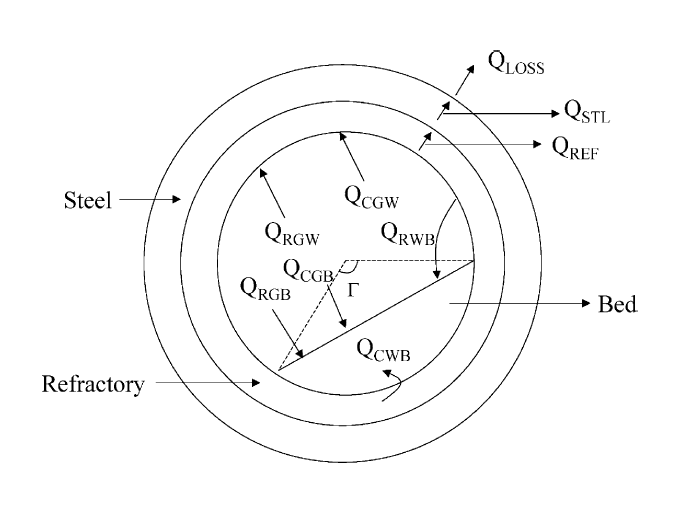
\includegraphics[width=0.5\linewidth]{media/heat-transfer-mujumdar-2006}
\caption{\label{fig:heat-transfer-modes}Heat transfer modes in cross-section~\cite{Mujumdar2006i}.}
\end{figure}

Since the present model is formulated for steady conditions, a set of constraints arising from the heat balances must be satisfied at each position along the kiln length. Performing the required balances based on Fig.~\ref{fig:heat-transfer-modes} one can find the following set of equations \eqref{eq:constraint-q1} to \eqref{eq:constraint-q4}. Because of inclusion of radiation phenomena and temperature dependent properties, these are intrinsically non-linear and an adapted solution method is to be chosen later. Addition of extra layers, \emph{e.g.} an internal air layer for energy recovery as proposed by \textcite{Mujumdar2006ii}, is straightforward for steady-state cases.

\begin{align}
Q_{coat}  &= Q_{CGW} + Q_{RGW} - Q_{RWB} - Q_{CWB}\label{eq:constraint-q1}\\
Q_{refr}  &= Q_{coat}\label{eq:constraint-q2}\\
Q_{shell} &= Q_{refr}\label{eq:constraint-q3}\\
Q_{env}   &= Q_{shell}\label{eq:constraint-q4}
\end{align}

Because plug-flow equation are formulated in a single coordinate derivative terms, heat fluxes are to be provided as unit length values. A differential length $\mathrm{d}z$ can be expressed as the ratio of cross-section area and perimeter, what allows for easy incorporation of varying transversal area in the problem. In this formulation the energy flux per unit area is multiplied by the heat exchange perimeter for each process, subscripts being the same as the fluxes. The following expression provides heat source term for freeboard

\begin{equation}
\dot{Q}_{f}
=\frac{Q_{CGW}}{A_{CGW}}P_{CGW}
+\frac{Q_{RGW}}{A_{RGW}}P_{RGW}
+\frac{Q_{CGB}}{A_{CGB}}P_{CGB}
+\frac{Q_{RGB}}{A_{RGB}}P_{RGB}
\end{equation}

\noindent{}and the next its homologous for bed

\begin{equation}
\dot{Q}_{b}
=\frac{Q_{CGB}}{A_{CGB}}P_{CGB}
+\frac{Q_{RGB}}{A_{RGB}}P_{RGB}
+\frac{Q_{CWB}}{A_{CWB}}P_{CWB}
+\frac{Q_{RWB}}{A_{RWB}}P_{RWB}
\end{equation}

Expressions for computing each of the required fluxes still need to be provided. These are postponed for the next section because in most cases, although physically-based, this expressions recur to engineering approximations and correlations, what is outside the scope of the underlining balance models developed here. It must be emphasized that this approach proposed by the sources~\cite{Mujumdar2006i,Hanein2017} do not enter in details of heat transfer from flames. Improvements could be done by incorporating the treatment provided by \textcite{Gorog1983}.

\section{Constitutive laws}

So far we have summarized balance equations for mass, species, and energy in the different components of a typical kiln. Other than ideal gas approximation for specific mass, no other constitutive laws allowing for the applied form of the equations was given. In this section we given focus on the different models used to compute heat fluxes, chemical reactions, and required thermophysical properties. The different heat fluxes introduced in section \ref{sec:energy-coupling} are detailed in what follows together with other models required to fulfill the representation of a rotary kiln.

\subsection{Internal heat exchanges}

These represent a summary of the parameters proposed by \textcite{Mujumdar2006i} and \textcite{Hanein2017} with a critical view and formulation aiming numerical implementation as treated by later sections. Heat transfer modes that occur in a kiln include \begin{inparaenum}[(i)]
    \item combustion flue gases heat-up the bed and walls by convection
    \item and radiation,
    \item internal refractory walls transfer energy to the bed also by conduction,
    \item but also emit energy through radiation to bed surface.
\end{inparaenum} The following paragraphs discuss some phenomenological laws proposed in the literature to model these phenomena, grouping them by heat transfer mode. The same subscript notation as previously used for heat fluxes is conserved for related variables.

\subsubsection*{Convective heat transfer}

Freeboard gas transfers heat to bed and walls by convection. The general formulation for this mode is given by \eqref{eq:q-cgx}, where the convective heat transfer coefficient $h_{CGX}$ must be computed by a suitable model, with $X\in\{W,B\}$ for walls and bed, respectively.

\begin{equation}
Q_{CGX} = h _{CGX}A_{CGX}\left(T_{G}-T_{X}\right)
\label{eq:q-cgx}
\end{equation}

% TODO track all papers using these expressions.
The expressions provided by \textcite{Tscheng1979} are often~\cite{Mujumdar2006i,Hanein2017} accepted to provide a quantitative heat flux for the different convection modes covered here. Instead of providing the equations already with coefficients, equation \eqref{eq:h-cgx} presents the parametric form based on axial and angular Reynolds numbers proposed by the authors~\cite{Tscheng1979}, what is intended as a pseudo-code for numerical implementation.

\begin{equation}
h _{CGX} = a_{0}\frac{k_g}{D_e}Re_{D}^{a_{1}}Re_{\omega}^{a_{2}}\eta^{a_{3}}
\quad\text{where}\quad
\begin{cases}
    Re_{D}      &= \dfrac{\rho{}u{}D_{e}}{\mu}\\[8pt]
    Re_{\omega} &= \dfrac{\rho{}\omega{}D_{e}^2}{\mu}\\[8pt]
    D_{e}       &= \dfrac{D}{2}\left[\dfrac{2\pi-2\theta+\sin(2\theta)}{\pi-\theta+\sin(\theta)}\right]\\[8pt]
    \eta        &= \dfrac{\phi-\sin(\phi)}{2\pi}
\end{cases}
\label{eq:h-cgx}
\end{equation}

In equation \eqref{eq:h-cgx} $\phi$ refers to the central angle in \eqref{eq:bed-area} and for better reading $2\theta=\phi$. Specific weight $\rho$, velocity $u$, and viscosity $\mu$ are those of the gas, while $\omega$ is the angular speed used in Kramers equation \eqref{eq:kramers}. The required parameters for bed and wall convective heat transfer coefficients are provided in Tab.~\ref{tab:coefficients-h-cgx}.

\begin{table}[h!]
\centering%
\caption{\label{tab:coefficients-h-cgx}Coefficients for equation \eqref{eq:h-cgx}.}
\begin{tabular}{
    c
    S[table-format=-1.2]
    S[table-format=-1.3]
    S[table-format=-1.3]
    S[table-format=-1.3]    
}
\toprule[2pt]
    
& $a_{0}$
& $a_{1}$
& $a_{2}$
& $a_{3}$
\\
\midrule[2pt]
$h _{CGB}$
& 0.46
& 0.535
& 0.104
& -0.341
\\[12pt]
$h _{CGW}$
& 1.54
& 0.575
& -0.292
& 0.000
\\
\bottomrule
\end{tabular}
\end{table}

\subsubsection*{Radiative heat transfer}

Radiative transfer from gas to both walls and bed surface is described by \textcite{Mujumdar2006i} as provided by \textcite{Hottel1967}, as given in \eqref{eq:q-rgx}, where $X\in\{W,B\}$ stands for wall and bed, respectively. Radiative properties of gas, emissivity $\varepsilon_{G}$, and absorptivity $\alpha_{G}$, are discussed later.

\begin{equation}
Q_{RGX} = \sigma{}A_{RGX}\varepsilon\left(\varepsilon_{G}T_{G}^4-\alpha_{G}T_{X}^4\right)
\qquad\text{where}\qquad{}
\varepsilon=\frac{1+\varepsilon_{X}}{2}
\label{eq:q-rgx}
\end{equation}

For the couple wall-bed, the expression proposed by \textcite{Mujumdar2006i} is replaced by that of \textcite{Hanein2017} as provided in \eqref{eq:q-rwb}. The view factor $F_{RWB}$ is set to unity here, what should be the case for a flat bed, what is not an unjustified approximation overall. This expression is valid if both the emissivities of bed $\varepsilon_{B}$ and refractory $\varepsilon_{W}$ are above 0.8, what is the case in most practical applications.

\begin{equation}
Q_{RWB} = \sigma{}A_{RWB}^{\star}\left(T_{W}^4-T_{B}^4\right)
\qquad\text{where}\qquad{}
A_{RWB}^{\star}=\left[
\frac{1-\varepsilon_{W}}{\varepsilon_{W}A_{RGW}}+
\frac{1}{F_{RWB}A_{RWB}}+
\frac{1-\varepsilon_{B}}{\varepsilon_{B}A_{RWB}}+
\right]^{-1}
\label{eq:q-rwb}
\end{equation}

\subsubsection*{Conductive heat transfer}

The last mode of heat exchange happening inside the kiln concerns the heat conduction from walls to bed. \textcite{Mujumdar2006i} proposes to use a convection-like formulation using the heat transfer coefficient by \textcite{Tscheng1979}, as in \eqref{eq:q-cwb}.

\begin{equation}
Q_{CWB} = h _{CWB}A_{CWB}\left(T_{W}-T_{B}\right)
\label{eq:q-cwb}
\end{equation}

\noindent{}where the apparent convection coefficient \eqref{eq:h-cwb-tscheng} is expressed in terms of thermal conductivity $k_{B}$ of bed, its specific mass $\rho_{B}$ and heat $c_{P,B}$, other parameters being already described.

\begin{equation}
h _{CWB}=11.6\frac{k_{B}}{A_{CWB}}\left[\frac{\omega{}R^2\phi}{\alpha_{B}}\right]^{0.3}
\qquad\text{where}\qquad{}
\alpha_{B}=\frac{k_{B}}{\rho_{B}c_{P,B}}
\label{eq:h-cwb-tscheng}
\end{equation}

This expression does not take into account the effects of particle size, gas film, nor is valid at high temperatures as intended here. To this end, following a recommendation by \textcite{Hanein2017}, we replace \eqref{eq:h-cwb-tscheng} by the equation provided by \textcite{Li2005} given in \eqref{eq:h-cwb}.

% TODO perform numerical analysis of the contribution of each term in eq to feed the discussion below regarding the extrapolation..
\begin{equation}
h _{CWB}=\left[
\frac{\chi{}d_{p}}{k_{g}}+
\frac{1}{2}\left(\frac{2k_{B}\rho_{B}c_{p}\omega}{\theta}\right)^{-\frac{1}{2}}
\right]^{-1}
\label{eq:h-cwb}
\end{equation}

In this expression a dimensionless effective gas film thickness $\chi$ obtained from an extension of penetration theory proposed by \textcite{Li2005} is introduced. For the present implementation, data extracted from figure 4 of that source~\cite{Li2005} is used to fit $\chi=B+(A-B)\exp(-kd_{p})$, with $A=0.3$, $B=0.095$, and $k=0.0045$. The value of $A$ and $B$ provide the bounds of $\chi$, while $k$ gives the decay rate fitting the aforementioned data. This expression is valid for particle sizes in range \SIrange{157.5}{1038}{\micro\meter}, but its extrapolation for lower values seem reasonable given the unavailability of better data. Finally, the bed equivalent conductivity is function of solids and freeboard properties given in the Maxwell model

\begin{equation}
k_{B}=k_{g}\frac{f_{sum}+2\Phi{}f_{diff}}{f_{sum}-1\Phi{}f_{diff}}
\quad\text{where}\quad
\begin{cases}
    f_{sum}  &= 2k_{g}+k_{s}\\[8pt]
    f_{diff} &= k_{s}-k_{g}
\end{cases}
\end{equation}

\noindent{}where $\Phi$ is the solids fraction in bed. Again, we have provided the equation is a more algorithmic way so that it resembles its numerical implementation.

\subsection{External heat exchanges}

Heat transfer losses to the environment $Q_{env}$ is computed through a convection-radiation expression encompassing a global convective heat transfer coefficient $h_{env}$ and shell emissivity $\varepsilon_{shell}$, as given in \eqref{eq:q-env}~\cite{Mujumdar2006i,Mujumdar2006ii}. The value of the convective heat transfer coefficient $h_{env}$ is assumed to be known and reasonable values are found to be typically in the range \SIrange{5}{25}{\watt\per\square\meter\per\kelvin}, depending on environmental conditions.

\begin{equation}
Q_{env}=A_{env}\left[
    h_{env}(T_{shell}-T_{env})
    +\sigma{}\varepsilon_{env}(T_{shell}^4-T_{env}^4)
\right]
\label{eq:q-env}
\end{equation}

Since all heat being exchanged with the environment results from radial conduction through kiln wall, the different layers need to be represented. This takes the form of a steady-state solution of heat equation for conduction across a hollow cylinder of length $l$ takes the form of \eqref{eq:q-radial}.

\begin{equation}
Q_{radial}
=2\pi{}lk\dfrac{(T_1-T_2)}{\ln\dfrac{r_2}{r_1}}
\label{eq:q-radial}
\end{equation}

Applying \eqref{eq:q-radial} to constraints \eqref{eq:constraint-q2} to \eqref{eq:constraint-q4} leads to \eqref{eq:radial-heat-flux}. In this expression the value of the different thermal conductivities are proposed to be computed as the average value in the respective material in the temperature range it is submitted to. The subscripts refer to the interfaces, $WI$ is the internal wall exposed surface, $CR$ is the coating-refractory interface, $RS$ the refractory shell interface. These expressions complete the constitutive heat transfer laws required to fulfill constraints from section \ref{sec:energy-coupling}.

\begin{equation*}
 k_{coat} \dfrac{(T_{WI}-T_{CR})}   {\ln\dfrac{R_{CR}}   {R_{WI}}}
=k_{refr} \dfrac{(T_{CR}-T_{RS})}   {\ln\dfrac{R_{RS}}   {R_{CR}}}
=k_{shell}\dfrac{(T_{RS}-T_{shell})}{\ln\dfrac{R_{shell}}{R_{RS}}}
=\frac{Q_{env}}{2\pi{}l}
\label{eq:radial-heat-flux}
\end{equation*}

\subsection{Freeboard kinetics}

Combustion in turbulent flows time-scales can be governed by mixing due to turbulent eddies. \textcite{Mujumdar2006i} proposes the use of eddy break-up model (EBU) to take this effect into account. In this approach, if the reaction rates  are faster than the value allowed by turbulent mixing, the later are taken into account, \emph{i.e.} $\dot{\omega}=\min\left(\dot{\omega}_{EBU},\dot{\omega}_{MAK}\right)$, where the subscript $MAK$ stands for mass action kinetics. For a one-step methane combustion model \ch{CH4 + 2 O2 -> CO2 + 2 H2O} we write

\begin{align}
\dot{\omega}_{EBU} &=
C_{R}\rho\dfrac{k}{\epsilon}\min\left[y_{F},\dfrac{y_{O}}{b}\right]\\
\dot{\omega}_{MAK} &=
k_{r}\rho^{2}y_{F}y_{O}\qquad\text{where}\qquad{}k_{r}=k_{0}\exp\left(-\frac{E_{a}}{RT}\right)
\end{align}

\noindent{}where fuel and oxidizer mass fractions are denoted $y_{F}$ and $y_{O}$, respectively, $C_{R}$ is an {EBU} parameter, often set to 4~\cite{Mujumdar2006i}, $E_{a}$ is the reaction activation energy. The ratio of turbulent kinetic energy to turbulent dissipation rate $\sfrac{k}{\epsilon}$ must be obtained from {CFD} simulations. In one dimension it is proposed~\cite{Mujumdar2006i} to approximate this ratio as the relative coordinate $z$ measured from the burner with respect to kiln length $L$, so $\sfrac{z}{L}$, but this hypothesis is considered too weak for practical use and {CFD} evaluations are required anyways~\footnote{For practical applications involving heat losses only, it is recommended to use an equivalent combustion flue gas evaluated from adiabatic flame conditions. This is not incompatible with freeboard-bed mass exchanges, if any.}.

\ifnotdraft
Parameter $b$

\begin{table}
\centering%
\caption{\label{tab:methane-combustion}Parameters for methane combustion rate expression.}
\end{table}
%\subsection{Pyrolysis and combustion of solids}
%\subsection{Bed kinetics}
\fi

\subsection{Drying of solids}

Drying of solids is not integrated in the more recent models considered in this study~\cite{Boateng1996,Mujumdar2006i,Mujumdar2006ii,Fan2013,Csernyei2016,Hanein2017,Shcherbina2019}, and is considered only in an oversimplified fashion in \textcite{Manitius1974}. The treatment provided by \textcite{Thurlby1988} is not applicable here since it handles pellets only. The implementation of this feature in the model is a work in progress.

\subsection{Physical properties}

\subsubsection*{Gas properties}

Thermophysical properties of gas species are those provided in Gri-Mech 3.0~\cite{Smith1999} and distributed in data files from Cantera~\cite{Goodwin2014}. In the case of transport properties, while a kinetic theory mixture-based implementation is unavailable, those reported by \textcite{Mujumdar2006i} are used.

\subsubsection*{Gas emissivity and absorptivity}

According to \textcite{Mujumdar2006i} the influence of \ch{CO2} and \ch{H2O} in flue gas over radiation properties of the mixture in their works~\cite{Mujumdar2006i,Mujumdar2006ii} was estimated from data provided in the work of \textcite{Gorog1981}, who recapitulates the approximations previously proposed by \textcite{Hottel1967} given in \eqref{eq:hottel-emissivity}, with a similar expression being used for absorptivity $\alpha_{G}$. In the present work we disagree that the data provided in the referred paper~\cite{Gorog1981} is enough to fit parameters for the end aimed by \textcite{Mujumdar2006i}, specially considering composition of fumes from natural gas flames.

\begin{equation}
    \varepsilon_{G}=\sum_i{}a_i\left[1-\exp\left(-k_i{}pr\right)\right]
    \qquad\text{with the constraint that}\qquad
    \sum_i{}a_1=1
    \label{eq:hottel-emissivity}
\end{equation}

Because effects of non-gray gas cannot be neglected in the presence of combustion products such as steam and soot~\cite{Tam2019}, an alternative approach is included in the present model. A first model for this end would be the weighted sum of gray gases, as reported by \textcite{Smith1982}, but it is not general enough for all applications. A better candidate is the {RADCAL} model by \textcite{Grosshandler1993}. Because of its complexity and details being beyond the scope of the present work, the reader is invited to consult its source report~\cite{Grosshandler1993}. \textcite{Tam2019,Yuen2009} have proposed neural network models trained to evaluate {RADCAL} and obtained with success values of gas emissivity $\varepsilon_{G}$ and absorptivity $\alpha_{G}$. Because no network coefficients are provided~\cite{Yuen2009} and numerical precision is insufficient in the other case~\cite{Tam2019}, we proceed with a new model fitting with a dense neural network.

% TODO this table is outdated
\begin{table}[h!]
    \centering%
    \caption{\label{tab:sample-space-radcal}Limits of sample space used to run {RADCAL}.}
    \begin{tabular}{ccccc}
        \toprule[2pt]
        Data set
        & Parameter
        & Minimum
        & Maximum
        & No. of points
        \\
        \midrule[2pt]
        \multirow{5}{*}{1}
        & Temperature (wall/gas)
        & \SI{300}{\kelvin}
        & \SI{2500}{\kelvin}
        & 10
        \\
        & Length
        & \SI{0.0}{\meter}
        & \SI{5.0}{\meter}
        & 6
        \\
        & \ch{CO} partial pressure
        & \SI{0.01}{\atm}
        & \SI{0.20}{\atm}
        & 5
        \\
        & \ch{CO2} partial pressure
        & \SI{0.01}{\atm}
        & \SI{0.20}{\atm}
        & 5
        \\
        & \ch{H2O} partial pressure
        & \SI{0.01}{\atm}
        & \SI{0.30}{\atm}
        & 5
        \\
        \midrule
        \multirow{5}{*}{2}
        & Temperature (wall/gas)
        & \SI{400}{\kelvin}
        & \SI{2400}{\kelvin}
        & 10
        \\
        & Length
        & \SI{0.1}{\meter}
        & \SI{4.9}{\meter}
        & 6
        \\
        & \ch{CO} partial pressure
        & \SI{0.02}{\atm}
        & \SI{0.19}{\atm}
        & 5
        \\
        & \ch{CO2} partial pressure
        & \SI{0.02}{\atm}
        & \SI{0.19}{\atm}
        & 5
        \\
        & \ch{H2O} partial pressure
        & \SI{0.02}{\atm}
        & \SI{0.29}{\atm}
        & 5
        \\
        \bottomrule
    \end{tabular}
\end{table}

%TODO provide model parameters/network details.
%TODO provide learning curve.

\section{Numerical solution}

\subsection{Solution approaches}

Presently, two different solution approaches were implemented. The nonlinear system of equations was solved both iteratively by a succession of separate solutions of freeboard, bed, and shell losses, with heat fluxes being relaxed at each step, or under the form of a single system of coupled non-linear equations. Numerical implementation was chosen to be supported by CasADi framework~\cite{Andersson2018} because of its automatic differentiation capabilities and interface for the solvers used with both solution approaches. Coupled system solution was carried out with help of Ipopt~\cite{Wachter2005} and was found to be the fastest approach.

%\subsection{Coupled solution}
%\subsection{Segregated solution}

In the case of uncoupled solution, the approach is interesting especially when combustion chemical kinetics at flame scale is to be solved during simulation. This is because of the numerical stiffness of kinetics which introduces a prohibitive mesh size for the coupled approach. In this case solution is performed with a {DAE} system solver provided by {SUNDIALS}~\cite{Hindmarsh2005} package for freeboard and solution points are recovered at cell centers for use in heat exchange calculations. Bed equations tend to be non-stiff and can be solved by a simple forward Euler or Runge-Kutta 4th order methods.

\subsection{Model validation}

The present model is not a direct implementation of any of the references upon which it was based. Nonetheless, it is possible to establish a parallel with conditions reported elsewhere~\cite{Barr1986PhD,Hanein2017}. Currently the only validation case available is the reproduction of condition T4 from \textcite{Barr1986PhD} which has also been simulated by \textcite{Hanein2017}. The overall agreement with the reference case is good, specially in what concerns the bed temperature, as it is depicted in figure \ref{fig:validation-barr}. The main difference here from the results by \textcite{Hanein2017} is the radiation model, what is an ongoing development.

\begin{figure}[!ht]
\centering
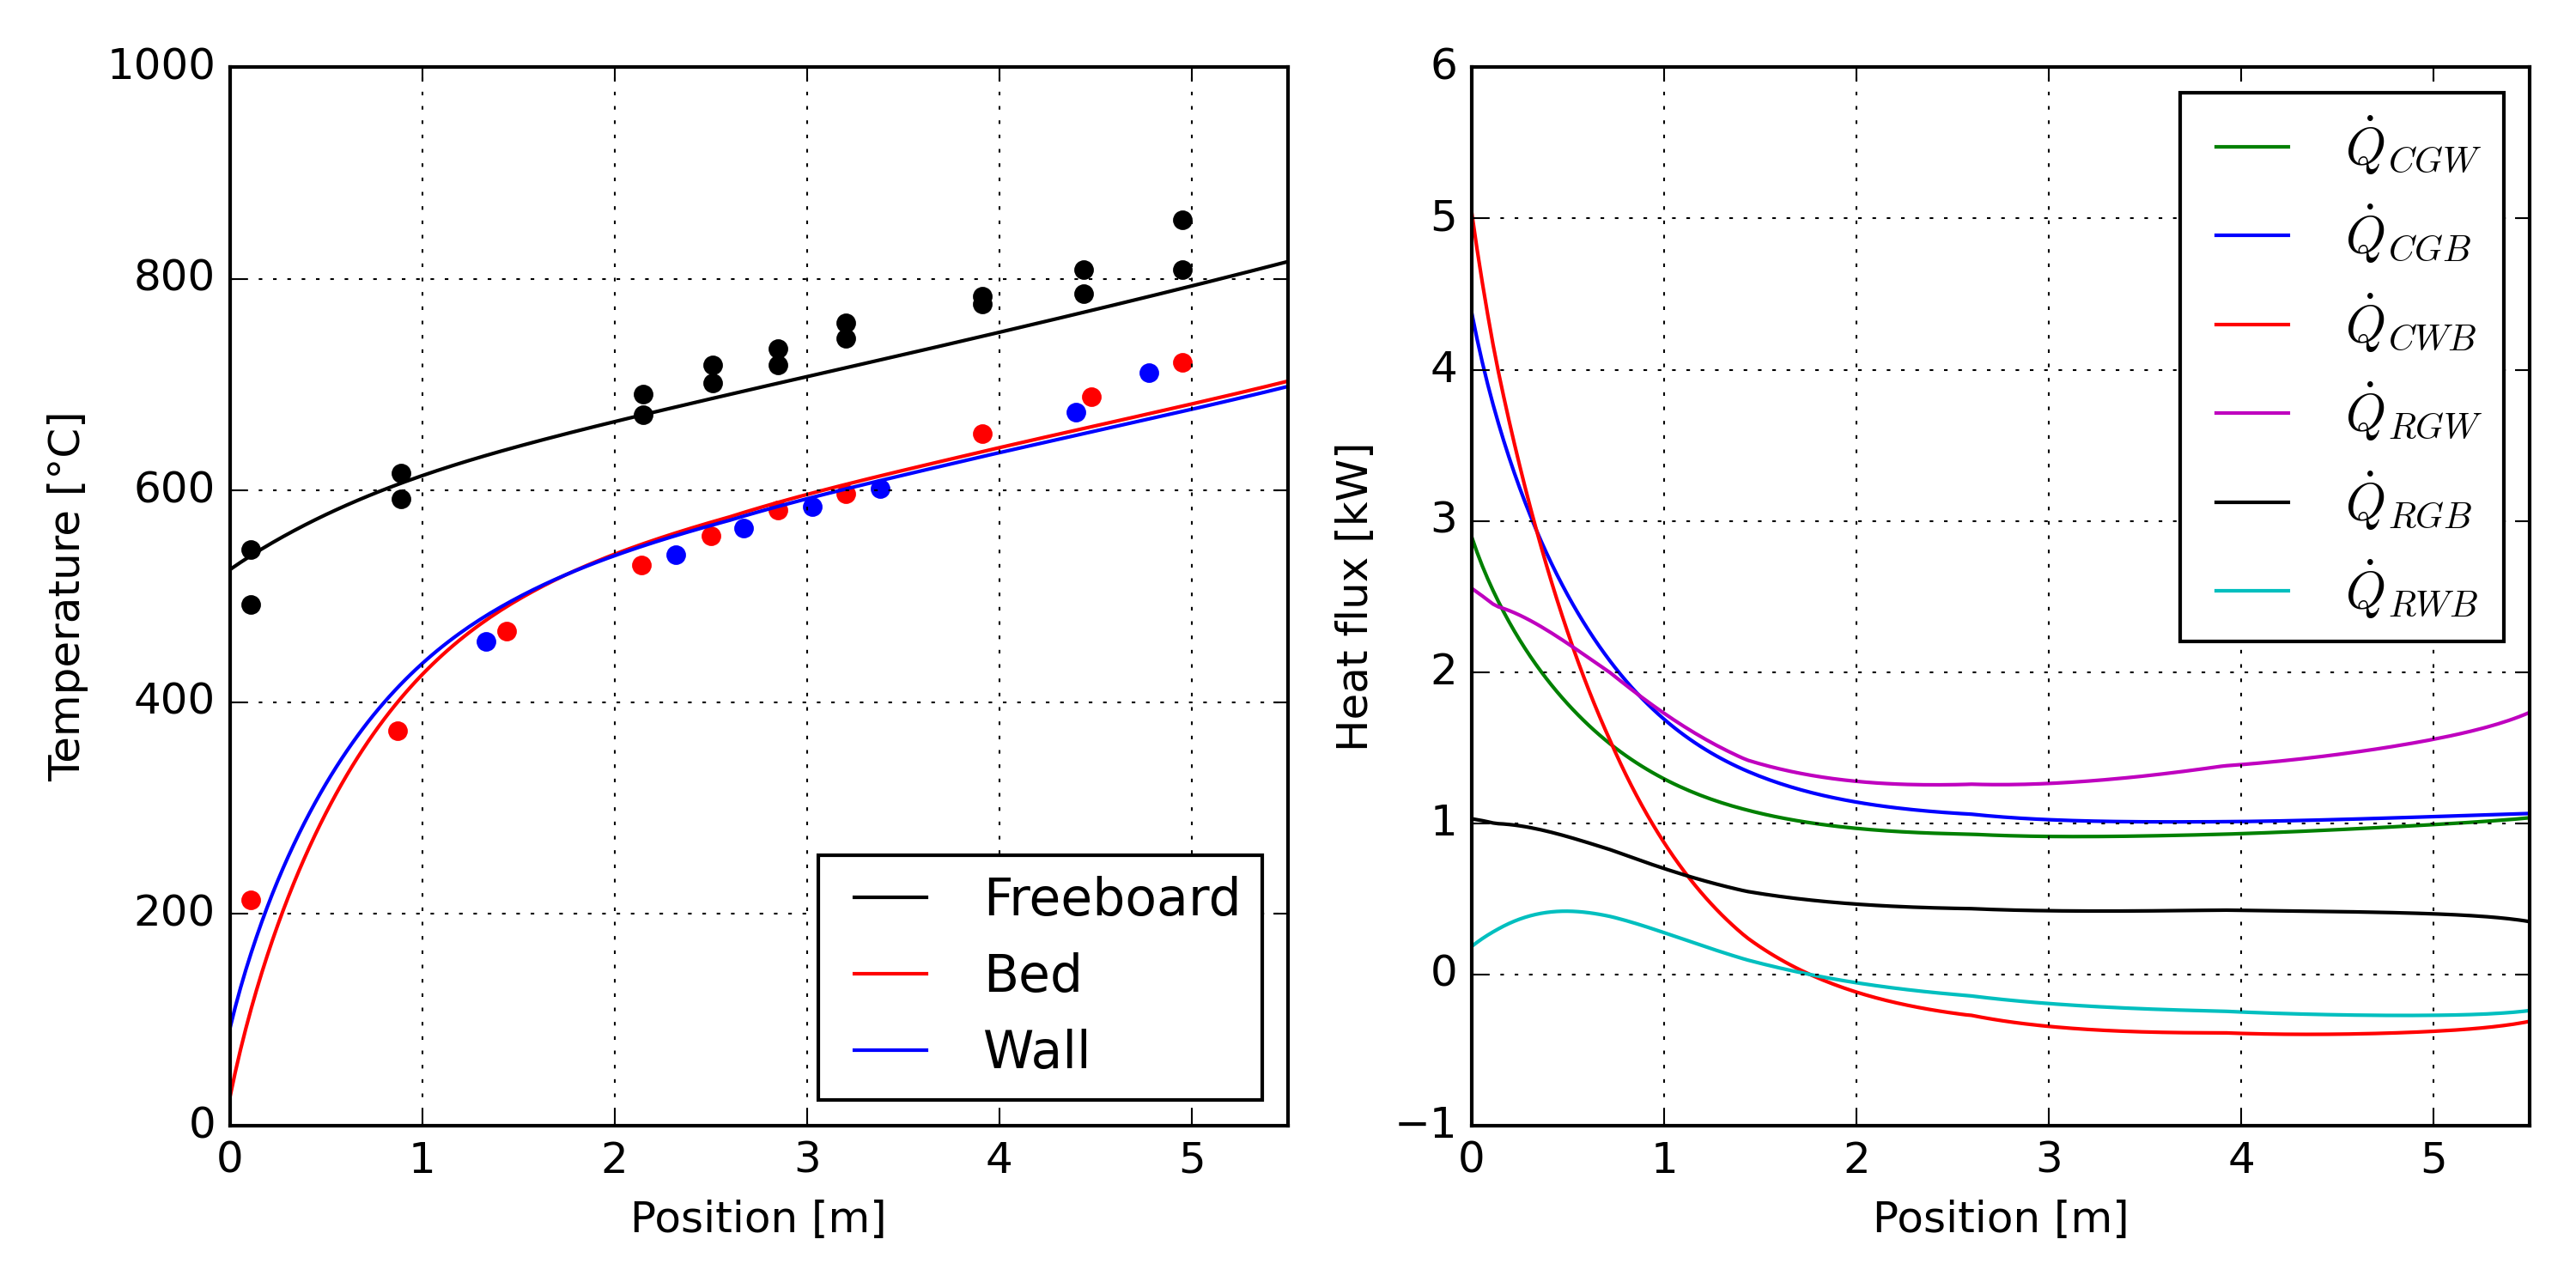
\includegraphics[width=0.95\linewidth]{media/validation-barr}
\caption{\label{fig:validation-barr}Results obtained with condition T4 from \textcite{Barr1986PhD}.}
\end{figure}

\ifnotdraft
\section{Results}
\fi

\section*{Conclusion}
\addcontentsline{toc}{section}{Conclusion}

An experimental rotary kiln model has been developed based on an extensive literature review. There seems to exist a general agreement that axial transport in a cement rotary kiln, in both freeboard and bed, can be represented by a plug-like model. This simplification allows for other phenomena to be taken into account in reasonable computation times, such as gas and bed kinetic transformations - not yet implemented in the present. The key elements for the accuracy of such a model are the constitutive relationships used to model the different energy transfer phenomena and materials properties. Semi-quantitative results are already possible for non-reacting materials, as demonstrated through the validation case. A road-map of features to be included in model was draft.

\clearpage%
\printbibliography%
\clearpage%
\listoftables%
\listoffigures%

\ifnotdraft%
\printunsrtglossary[type=symbols,style=long]%
\fi%

\clearpage%

\appendix%
\section{User guide}

\subsection{Configuration file}

Most values are to be provided in SI units but since a few exceptions exist, units are provided in all cases where applicable. The entries present on the different sub-dictionaries of this file are described below. All keys must respect the case as indicated.

\noindent{}Elements under sub-dictionary \mintinline{json}+"geometry"+

\begin{itemize}
    \item \mintinline{json}+"kiln_slope"+
    kiln global slope in degrees [\si{\degree}].
    
    \item \mintinline{json}+"kiln_inner_length"+
    kiln total internal length in meters [\si{\meter}].
    
    \item \mintinline{json}+"kiln_inner_diameter"+
    kiln refractory inner diameter [\si{\meter}].
    
    \item \mintinline{json}+"kiln_dam_height"+
    height of dam at kiln discharge [\si{\meter}].
    
    \item \mintinline{json}+"thickness_refractory"+
    thickness of refractory layer [\si{\meter}]. Provide a negative value for enabling use of function implementation (see below).
    
    \item \mintinline{json}+"thickness_shell"+
    thickness of kiln external metallic shell [\si{\meter}]. Provide a negative value for enabling use of function implementation (see below).
    
    \item \mintinline{json}+"thickness_coating"+
    thickness of inner coating (formed by agglomeration/melting of processed material) [\si{\meter}]. In most cases this variable is to be provided through a position dependent function as described in the next section. Provide a negative value for enabling use of function implementation (see below).
\end{itemize}

\noindent{}Elements under sub-dictionary \mintinline{json}+"operation"+

\begin{itemize}
    \item \mintinline{json}+"rotation_rate"+
    kiln rotation rate [rev/min].
    
    \item \mintinline{json}+"bed_feed_rate"+
    bed material feed rate [\si{\kilo\gram\per\hour}].
    
    \item \mintinline{json}+"gas_flow_rate"+
    mixture of natural gas plus primary air flow rate [\si{\kilo\gram\per\second}].
    
    \item \mintinline{json}+"gas_leak_rate"+
    secondary air flow entering the kiln through discharge [\si{\kilo\gram\per\second}].
    
    \item \mintinline{json}+"bed_feed_temperature"+
    temperature of bed material at feed point [\si{\kelvin}].
    
    \item \mintinline{json}+"gas_feed_temperature"+
    temperature of global gas inlet [\si{\kelvin}]. This property is still controversial because the mixing of combustion gases and secondary air coming from discharge is not yet implemented. For now the user is recommended to use a Python script to pre-process gas flows and temperature.
    
    \item \mintinline{json}+"bed_feed_humidity"+
    mass percentage of water in bed feed [\%].
    
    \item \mintinline{json}+"gas_feed_composition"+
    array of species mole fractions [-]. Again, this is the resulting composition from mixing of combustion gases and leak. See the \mintinline{json}+"gas_feed_temperature"+ for recommendations.
\end{itemize}

\noindent{}Elements under sub-dictionary \mintinline{json}+"initial_guess"+

\begin{itemize}
	\item \mintinline{json}+"gas_final_temperature"+
	expected final gas temperature at fumes outlet for initialization [\si{\kelvin}].
	
	\item \mintinline{json}+"bed_final_temperature"+
	expected final bed temperature at material discharge for initialization [\si{\kelvin}].
\end{itemize}

\noindent{}Elements under sub-dictionary \mintinline{json}+"heat_transfer_parameters"+

\begin{itemize}
	\item \mintinline{json}+"emissivity_bed"+
	bed material emissivity [-]. Typically in range 0.80-0.90.
	
	\item \mintinline{json}+"emissivity_refractory"+
	refractory material emissivity [-]. Typically in range 0.80-0.90.
	
	\item \mintinline{json}+"emissivity_shell"+
	shell material emissivity [-]. Typically 0.79 for corroded steel.
	
	\item \mintinline{json}+"environment_htc"+
	environment heat transfer coefficient [\si{\watt\per\square\meter\per\kelvin}].
	
	\item \mintinline{json}+"environment_temperature"+
	environment temperature [\si{\kelvin}].
	
	\item \mintinline{json}+"conductivity_coating"+
	thermal conductivity of internal coating material [\si{\watt\per\meter\per\kelvin}]. Provide a negative value for enabling use of function implementation (see below).
	
	\item \mintinline{json}+"conductivity_refractory"+
	thermal conductivity of refractory material [\si{\watt\per\meter\per\kelvin}]. Provide a negative value for enabling use of function implementation (see below).
	
	\item \mintinline{json}+"conductivity_shell"+
	thermal conductivity of shell material [\si{\watt\per\meter\per\kelvin}]. Provide a negative value for enabling use of function implementation (see below).
\end{itemize}

\noindent{}Elements under sub-dictionary \mintinline{json}+"hypothesis"+

\begin{itemize}
	\item \mintinline{json}+"gas_equilibrated"+
	if true, gas kinetics is disabled. Enabling this accelerates computations through coarser meshes and is generally the best practice. For preparing the equivalent composition use a Python script.
	
	\item \mintinline{json}+"gas_kinetics"+
	a choice between eddy break-up model \mintinline{json}+"EBU"+ or mass action kinetics \mintinline{json}+"MAK"+. Under natural gas conditions used in a rotary kiln it is recommended to use\mintinline{json}+"EBU"+.
	
	\item \mintinline{json}+"gas_film_thickness"+
	dimensionless thickness of gas film used in gas-bed heat transfer coefficient estimation. For more details on how to set this value, please refer to \href{https://doi.org/10.1002/ceat.200500241}{Li (2005)} and \href{https://doi.org/10.1080/17436753.2017.1303261}{Hanein (2017)}.
\end{itemize}

\noindent{}Elements under sub-dictionary \mintinline{json}+"numerical"+

\begin{itemize}
	\item \mintinline{json}+"number_of_slices"+
	number of slices (cells) in mesh.

	\item \mintinline{json}+"discretization_method"+
	presently only `"linear"` discretization is allowed.
\end{itemize}

\noindent{}Elements under sub-dictionary \mintinline{json}+"ipopt"+ are parameters provided to Ipopt nonlinear solver. In listing \ref{listing:configuration-file} the most common attributes used with the present model are provided. For a full list check \href{https://coin-or.github.io/Ipopt/OPTIONS.html}{Ipopt documentation}.

\noindent{}Elements under sub-dictionary \mintinline{json}+"materials"+ can be tweaked through the configuration file, which also acts as a database. More on the current status is provided below in the section dedicated to materials properties.

\begin{itemize}
	\item \mintinline{json}+"gas_data"+
	edition of gas data is currently not supported. Currently gas phase model is quite restrictive and only a 6-species methane combustion model is accepted. Kinetics and transport properties are hardcoded and modifying it require changes to GasMixture class provided with the package. Thermophysical properties can be configured through a JSON file provided in the data folder using NASA-7 polynomial coefficients, but that represents little interest because the current values are the well accepted ones extracted from a Gri-Mech 3.0 version provided with Cantera.
	
	\item \mintinline{json}+"bed_data"+
	bed data is currently not documented. An example of user defined setup is provided in listing \ref{listing:project-data}.
\end{itemize}

Listing \ref{listing:project-data} below provide a practical configuration file used for model validation against reference results provided by \textcite{Hanein2017}.

\inputminted{json}{../sample/minified-for-dist/case-hanein-paper/simulate.json}
\captionof{listing}{\label{listing:configuration-file}Example of configuration file.}

\subsection{Configuration class}

For the arguments that can be position and/or temperature dependent, a class \mintinline{octave}+ProjectData+ with the interface provided below must be implemented and placed in the path of the simulation script. It must be noted that not all methods are required, but only those for which a valid value is not provided in the JSON configuration file. It must be emphasized that environment heat transfer coefficient and temperature shall be supplied with the same shape as coordinates array \mintinline{octave}+z+ for compatibility with setup.

\inputminted{octave}{../sample/minified-for-dist/case-hanein-paper/ProjectData.m}
\captionof{listing}{\label{listing:project-data}Example of ProjectData class definition.}

\subsection{Calling the model}

Calling the model can be done by the simplified API as provided in listing \ref{listing:method-one} of with direct manipulation of the model, as in listing \ref{listing:method-two}. In both cases we start by adding the required tools to the script path, them importing the packages prior to model setup and run. If you are using \mintinline{octave}+ProjectData+, this configuration assumes it is found under the same directory as the simulation script, otherwise you should add it to the path. This might be interesting when a conditional evaluated in the script require a variant of \mintinline{octave}+ProjectData+, and since duplicate file names are not possible this must be resolved through a directory structure.

\inputminted[firstline=11,lastline=21]{octave}{../sample/minified-for-dist/case-hanein-paper/simulate.m}
\captionof{listing}{\label{listing:method-one}Example of simulation script with wrapper API.}

\inputminted[firstline=11,lastline=23]{octave}{../sample/minified-for-dist/case-kiln-alumina/simulate.m}
\captionof{listing}{\label{listing:method-two}Example of simulation script with direct model call.}

\end{document}
